\section{数据、任务与探索性分析}
\label{sec:v2-data}

\subsection{数据来源、观测单位与预测目标}
本研究使用课程提供的 \texttt{data\_2026.csv}。一条记录对应某种药物在指定溶剂和温度条件下的一次溶解度观测。表\ref{tab:v2-data-fields}概括原始字段及其用途。预测输入为药物结构、溶剂结构和温度，目标为表中的 $y=\texttt{Solubility\_log10}$。训练和评价直接使用该对数尺度。系统在显示浓度时按 CSV 的单位字段将 $10^{\hat y}$ 解释为 mol/L。原文件未标注温度单位，温度特征和响应图均沿用 CSV 原始数值尺度。

\begin{table}[htbp]
  \centering\small
  \caption{课程数据字段与建模用途。全量 CSV 含 1904 条记录。}
  \label{tab:v2-data-fields}
  \begin{tabularx}{\linewidth}{@{}lX@{}}
    \toprule
    原始字段 & 含义与用途 \\
    \midrule
    \texttt{Drug}、\texttt{Solvent} & 药物和溶剂名称，用于展示和查找记录。 \\
    \texttt{Drug SMILES}、\texttt{Solvent SMILES} & 分子结构，用于计算描述符和构造分组键。 \\
    \texttt{Temperature} & 温度原始数值，用于刻画测量条件。 \\
    \texttt{Solubility\_log10} & 十进制对数溶解度，用于拟合和评价。 \\
    \texttt{Solubility Unit} & 原尺度的记录单位，全部为 mol/L。 \\
    \bottomrule
  \end{tabularx}
\end{table}

\subsection{结构标准化与数据质量处理}
使用 RDKit 解析 SMILES，将规范化后的完整药物与溶剂结构拼接为组合键。原表有 186 个药物名称，规范化后有 168 种完整药物结构和 49 种溶剂结构，其中 17 种完整药物结构对应多个名称。另以 \texttt{ChargeParent} 标准化药物并移除立体标记，得到 161 个药物母体。部分盐形式和立体变体因此进入同一组。基础描述符和丰富描述符均由各条记录的完整分子计算，母体键用于数据划分、训练计权和评价，标准化母体结构也作为丰富树的一种候选特征来源。

原始结构字段均可解析，模型输入与目标字段未发现缺失。按七个原始字段检查，发现 4 条额外的完全重复记录。以规范化的组合键和温度识别同条件观测，有 86 组、205 条记录出现不同溶解度标签，其中 11 组的标签极差超过 1 个对数单位。主实验保留这些记录及其原始标签。同一组合的记录随母体一起划分，重复记录不会跨越训练和验证边界。

在 1507 条开发记录上，以四分位距 $\mathrm{IQR}=Q_3-Q_1$ 标记越过 $[Q_1-1.5\,\mathrm{IQR},\,Q_3+1.5\,\mathrm{IQR}]$ 的观测。温度界限为 $[10,50]$，标记 228 条记录；目标界限约为 $[-4.633,2.599]$，标记 11 条记录。保留这些观测以覆盖较少见的条件和溶解度范围。生成的丰富描述符另行检查非有限值，插补量和特征筛选条件在相应训练折内确定。

\subsection{采样分布与条件覆盖}
在 $168\times49$ 个完整结构组合中，有 646 个在数据中出现，覆盖率为 7.85\%。其中 222 个组合有多条观测，合计占全部记录的 77.73\%。母体频次同样不均匀，74 个母体各有 1--5 条记录，共 182 条；30 个母体各有超过 20 条记录，共 1078 条。图\ref{fig:v2-data-overview}展示了组合覆盖与频次。全量温度介于 $-59.5$ 与 130，中位数为 25，目标介于 $-6.2343$ 与 $2.2168$。开发集中有 157 个组合的温度发生过变化，覆盖 73 个母体和 1118 条记录。

\begin{figure}[htbp]
  \centering
  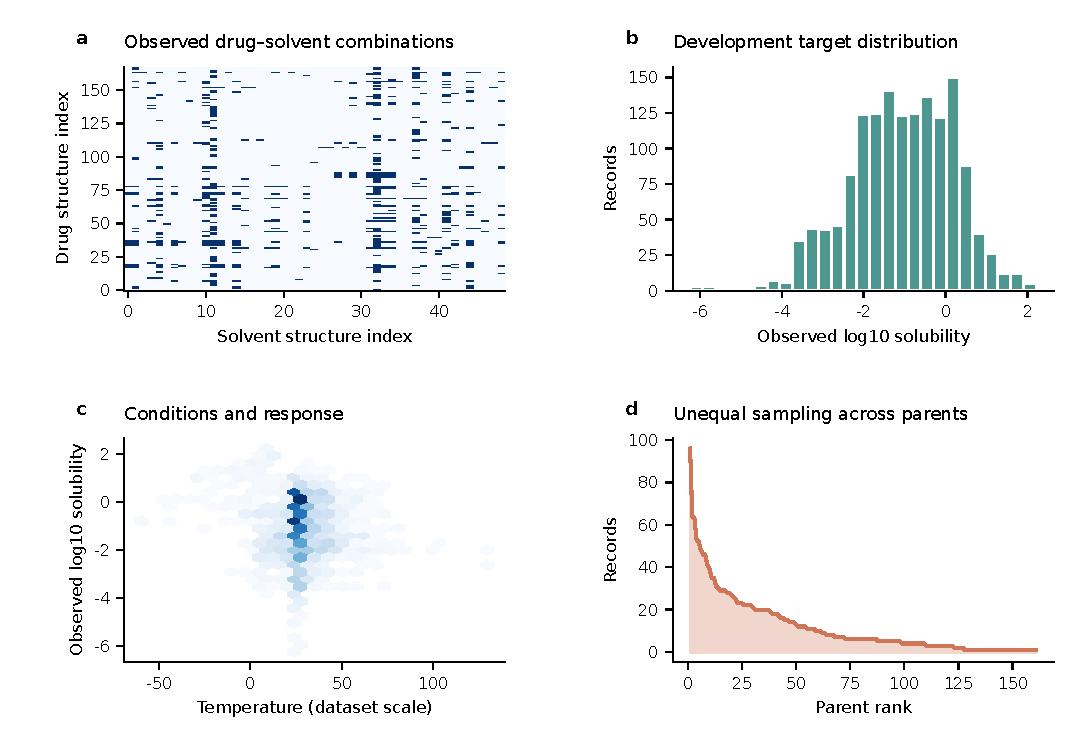
\includegraphics[width=\linewidth]{revision_v2/v2_data.pdf}
  \caption{数据覆盖、条件分布与采样频次。\textbf{a} 全量数据中观测到的完整药物与溶剂结构组合。\textbf{b,c} 开发集 1507 条记录的观测溶解度分布和温度与溶解度联合分布，颜色表示记录密度。\textbf{d} 全量数据的 161 个药物母体按观测数量排序。}
  \label{fig:v2-data-overview}
\end{figure}

\subsection{数据现象与设计假设}
有限的组合覆盖要求模型利用不同分子之间可比较的结构信息，因此后续比较基础描述符、丰富描述符与人工构造的药物--溶剂交互特征。母体频次不均意味着逐行平均误差更多反映高频母体的表现，因此将母体等权平均绝对误差作为主指标，并检验训练时采用母体加权的作用。存在温度变化的重复组合为组合内关联分析提供了观测基础，用于考察温度与溶解度在同一结构条件下如何共同变化。
